\documentclass[addpoints]{exam}
\usepackage[utf8]{inputenc}
\usepackage{amsmath}
\usepackage{tikz}
\usepackage{pgfplots}
\usetikzlibrary{datavisualization}
\usetikzlibrary{calc}
\usetikzlibrary{arrows}
\usetikzlibrary{decorations.pathreplacing,decorations.markings}
\usetikzlibrary{datavisualization.formats.functions}
\usepackage[american,siunitx]{circuitikz}
\ctikzset{bipoles/resistor/width=.35}
\ctikzset{bipoles/resistor/height=.15}
\pgfplotsset{width=3cm,compat=1.4}
\usepackage{graphicx}%
\usepackage{mathtools}
\usetikzlibrary{arrows,shapes,positioning}
\usetikzlibrary{decorations.markings}
\tikzstyle arrowstyle=[scale=1]
\tikzstyle directed=[postaction={decorate,decoration={markings,
    mark=at position .65 with {\arrow[arrowstyle]{stealth}}}}]
\tikzstyle reverse directed=[postaction={decorate,decoration={markings,
    mark=at position .65 with {\arrowreversed[arrowstyle]{stealth};}}}]
\usepackage{dirtytalk}
\usepackage{relsize}
\graphicspath{ {images/} }
\DeclarePairedDelimiter{\ceil}{\lceil}{\rceil}
\usepackage{geometry}
\usepackage{draftwatermark}
\SetWatermarkFontSize{2cm}
\SetWatermarkText{DU-Physics}
\usepackage[banglamainfont=Kalpurush, 
            banglattfont=Siyam Rupali
           ]{latexbangla}
        
\begin{document}
\begin{LARGE}
\begin{center}
পদার্থবিজ্ঞান (Physics - 2009)
\end{center}
\end{LARGE}
\begin{questions}

\question যদি $ \vec{P} = 2\hat{i}+4\hat{j}-5\hat{k} $ এবং $ \vec{Q} = \hat{i}+2\hat{j}+3\hat{k} $ হয় তবে এদের মধ্যবর্তী কোণ -  (If $ \vec{P} = 2\hat{i}+4\hat{j}-5\hat{k} $ and $ \vec{Q} = \hat{i}+2\hat{j}+3\hat{k} $ then the angle between them is -  )

\begin{oneparchoices}
\choice $ 78.1^{\circ} $
\choice $ 105.25^{\circ} $
\choice $ 11.49^{\circ} $
\choice $ 101.49^{\circ} $
\end{oneparchoices}

 \question  একটি নল থেকে পানি বের হয়ে $ 2\,ms^{-1} $ বেগে একটি দেয়ালকে লম্বভাবে আঘাত করছে। নলের প্রস্থছেদ হচ্ছে $ 0.03\,m^{2} $। ধরা যাক পানি দেয়াল থেকে রিবাউনড করছে না। দেয়ালের উপর পানি কি পরিমাণ বল প্রয়োগ করছে? (পানির ঘনত্ব $ 1000\,kg/m^{3} $) (Water emergest at $ 2\,ms^{-1} $ from a pipe and hits a wall at right angles. The pipe has a cross sectional area of $ 0.03\,m^{2} $. Calculate the force on the wall assuming that the water does not rebound.) (Density of water = $ 1000\,kg/m^{3} $)

\begin{oneparchoices}
\choice 1000 N
\choice 300 N
\choice 120 N
\choice 240 N
\end{oneparchoices}

\question নিন্মলিখিত বর্তনীর সমতুল্য রোধ কোনটি? (What is the equivalent resistance of the following circuit?)

 \begin{center}
\begin{circuitikz}\draw
        (0,3) to[R=$R$] (0,1.5)to[R=$R$](0,0)--(3,0);
      \draw  (1.5,0)to[R=$R$](1.5,1.5)to [R=$R$](1.5,3);
      \draw (0,3)--(3,3)to[battery1](3,0);
    \end{circuitikz}
 \end{center}

\begin{oneparchoices}
\choice $4$ R
\choice R
\choice $ \dfrac{3}{4}$ R
\choice None

\end{oneparchoices}

\question  একটি কাঁচ পৃষ্ঠের উপর পানি ঢাললে তা যতটুকু ছড়ায় দুধ ততটা ছড়ায় না। এর কারণ- (If water is poured on aglass surface is splashes. However milk does not splash so much. The reason is-)

\begin{oneparchoices}
\choice সান্দ্রতা (viscosity)
\choice পৃষ্ঠটান (surface tension)
\choice Both
\choice None
\end{oneparchoices}

\question  একটি বৈদ্যুতিক পাখার সুইচ \say{অন} করলে দশবার পূর্ণ ঘূর্ণনের পর পাখাটির কৌণিক বেগ হয় 20 rad/s। কৌণিক ত্বরণ কত? (If the switch of an electric fan is turned \say{on} the angular velocity of the fan is 20 rad/s after 10 complete cycle. What is the angular acceleration ?) 

\begin{oneparchoices}
\choice $ 1.8\,rad/s^{2} $
\choice $ 8.13\,rad/s^{2} $
\choice $ 3.18\,rad/s^{2} $
\choice $ 5.17\,rad/s^{2} $

\end{oneparchoices}


\question  256 cycles/s কম্পাংক বিশিষ্ট একটি সুর শলাকা হতে উৎপন্ন শব্দ তিন সেকেন্ডে 1020 m দূরত্ব অতিক্রম করে। বায়ুতে শব্দের তরঙ্গ দৈর্ঘ্য কত? (The sound produced by tuning fork with frequency 256 cycles/s travels 1020 m is seconds. What is the wave length of sound in air?)

\begin{oneparchoices}
\choice  132.8 m
\choice  308.7 m
\choice  132.8 cm
\choice  225.5 cm
\end{oneparchoices}

\question $ 1\mu F,\, 2\mu F$ এবং $ 3\mu F $ ধারকত্ব বিশিষ্ট তিনটি ধারককে শ্রেণীসমবায়ে যুক্ত করা হল। এদের তুল্য ধারকত্ব কত হবে? (Three capacitors of values $ 1\mu F,\, 2\mu F$ and $ 3\mu F $ are connected in series. The equivalent capacitance would be - ) 

\begin{oneparchoices}
\choice $ 7\mu F $
\choice $ 2.3\mu F $
\choice $ 1.75\mu F $
\choice $ 0.57\mu F $

\end{oneparchoices}

\question  $ 900kg $ ভরের একটি ট্রাক ঘণ্টায় $ 60\,km $ বেগে চলছে। ব্রেক চেপে ট্রাকটি 50 মিঃ দূরে থামানো হল। যদি মাটির ঘর্ষণ জনিত বল $ 200\,N $ হয় তবে ব্রেক জনিত বলের মান কত? (A truck weighing $ 900kg $ travels with a velocity of $ 60\,km/h $ By applying brakes the truck was stopped 50 m away. If the frictional force of soil is . What is the force applies by the brakes?) 

\begin{oneparchoices}
\choice $ 2300\,N $
\choice $ 2700\,N $
\choice $ 2500\,N $
\choice $ 2400\,N $

\end{oneparchoices}

\question  একটি ইয়ং এর দ্বি-চির পরীক্ষায় চিরদ্বয়ের মধ্যবর্তী দূরত্ব । চির থেকে দুর দূরতে ডোরার বেবধান 

\begin{oneparchoices}
\choice 70.7 Ampere
\choice 100 Ampere
\choice 50 Ampere
\choice 200 Ampere
\end{oneparchoices}


\question  সরলদোল গতি সম্পন্ন একটি কণার বিস্তার $ 0.02\,m $ এবং কম্পাংক $ 2.5\,Hz $ হলে এর সর্বোচ্চ দ্রুতি কত হবে? (What is the maximum speed of a particle having simple harmonic motion of amplitude $ 0.02\,m $ and frequency $ 2.5\,Hz $ ?)

\begin{oneparchoices}
\choice $ 0.05\,ms^{-1} $
\choice $ 0.125\,ms^{-1} $
\choice $ 0.157\,ms^{-1} $
\choice $ 0.314\,ms^{-1} $
\end{oneparchoices}

\question 50N এর একটি আনুভূমিক বল $ 0.5\,kg $ ভরের আয়াতাকার বস্তুকে উলম্ব দেয়ালে ধাক্বা দিচ্ছে । বস্তুটি আদতে স্থির ছিল। যদি স্থৈতিক ও গতীয় ঘর্ষণ গুনাঙ্ক যথাক্রমে $ \mu_{s} = 0.6 $ ও  $ \mu_{k} = 0.8 $ হয়, তবে $ m/s^{2} $ এককে বস্তুটির ত্বরণ কত? (A horizontal force of 50N pushes a 0.5kg rectangular body against a vertical wall. The body was initially at rest. If the static and kinetic co-efficient of friction are $ \mu_{s} = 0.6 $ and $ \mu_{k} = 0.8 $, respectively then what is the acceleration of the body in units of $ m/s^{2} $ ? )

\begin{oneparchoices}
\choice 1.8
\choice 2.0
\choice 6.0
\choice 8.0
\end{oneparchoices}

\question  একটি তারের ভিতর দিয়ে সাইনুসয়ডাল তরঙ্গ প্রবাহিত হলে তারের কণার সর্বোচ্চ দ্রুতি $ v_{s} $ । তারের একটি কণার সরণ সবোর্চ্চ সরণের অর্ধেক হলে ঐ কণার দ্রতি হলো - (The maximum speed of particle of a string carrying a sinusoidal wave is $ v_{s} $. When the displacement of the particle on the spring is half of its maximum, its speed is: )

\begin{oneparchoices}
\choice $ \dfrac{v_{s}}{2} $
\choice $ \dfrac{\sqrt{3}v_{s}}{2} $
\choice $ 2v_{s} $
\choice $ \dfrac{2v_{s}}{4} $
\end{oneparchoices}

\question  একটি নিউক্লিয়াস একটি নিউট্রন গ্রহন করে একটি বিটা কণা $ (\beta^{-})  $ নি:সরণ করে  দুটি আলফা কণায় পরিণত হয় । আদি নিউক্লিয়াসের A এবং Z যথাক্রমে ছিল - (A certain nuclues after absorbing a neutron, emits a beta $ (\beta^{-})  $ particle and then splits into two alpha particles. The A and Z respectively of the original nucleus were:)

\begin{oneparchoices}
\choice 6
\choice 7, 2
\choice 7, 3
\choice 8, 4
\end{oneparchoices}

\question  $ e $ মানের একটি চার্জ $ r $ ব্যাসার্ধের একটি বৃত্তাকার পথে $ v $ দ্রুতিতে ঘুরছে। বৃত্তের কেন্দ্রে চৌম্বকক্ষেত্রের মান হবে:  (A charge of magnitude $ e $ is traveling with speed $ v $ in circular path of radius $ r $. The magnitude of the magnetic field at the center of the circle is: )

\begin{oneparchoices}
\choice  $\dfrac{\mu_{0}ev}{4\pi r^{2}}$
\choice  $\dfrac{\mu_{0}ev}{2\pi r}$
\choice  $\dfrac{\mu_{0}ev}{\pi r^{2}}$
\choice  $\dfrac{\mu_{0}ev}{4\pi v r}$
\end{oneparchoices}

\question  কৌণিক ভরবেগের একক কোনটি ? (Which is the unit of angular momentum?)

\begin{oneparchoices}
\choice $ kgm^{2}s^{-1} $
\choice $ kgms^{-2} $
\choice $ kgms^{-1} $
\choice $ kgm^{2}s^{-2} $

\end{oneparchoices}

\question  $ 10110101_{2} $ বাইনারি সংখ্যা হতে $ 10011_{2} $ বাইনারি সংখ্যা এর বিয়োগফল হলো (The binary found after subtracting $ 10011_{2} $ from the binary number $ 10110101_{2} $ is )

\begin{oneparchoices}
\choice $ 10110010_{2} $
\choice $ 10100010_{2} $
\choice $ 10100101_{2} $
\choice $ 10100011_{2} $

\end{oneparchoices}


\question  উৎস হতে ধ্বনিত শব্দ একজন ব্যাক্তি শুনতে পেল $ 5s $ পরে, যখন একই শব্দ আরেকজন ব্যাক্তি শুনতে পেল $ 6s $ পরে। শব্দের বেগ $ 300\,m/s $ । এই দুই ব্যাক্তির মধ্যে সবোর্চ্চ এবং সর্বনিন্ম দুরত্ব কত? (Sound produced from a source heard by a person after 5 seconds, while the same sound is heard by another person after 6 seconds. The speed of sound is $ 300\,m/s  $. What are the maximum and minimum distances, respectively between two persons?)

\begin{oneparchoices}
\choice $ 1.8\,km,\; 0.15\,km$
\choice $ 2.2\,km,\; 0.20\,km $
\choice $ 2.8\,km,\; 0.25\,km $
\choice  $ 3.3\,km,\; 0.30\,km $
\end{oneparchoices}



\question  তিনটি ভেক্টর $ \vec{a},\; \vec{b} $ ও $ \vec{c} $ যাদের মান যথাক্রমে ৪, ৩  এবং ৫, যোগ করলে শূণ্য হয় অর্থাৎ $ \vec{a}+\vec{b}+\vec{c} =0  $। তাহলে এর মান $ |\vec{c}\times (\vec{a}\times \vec{b})| $ হলো : (Three vectors $ \vec{a},\; \vec{b} $ and $ \vec{c} $ of magnitudes 4, 3 and 5, respectively add to zero i.e $ \vec{a}+\vec{b}+\vec{c} =0  $ then the value of $ |\vec{c}\times (\vec{a}\times \vec{b})| $ is:)

\begin{oneparchoices}
\choice 12
\choice 60
\choice 25
\choice 15
\end{oneparchoices}

\question  নিন্মের কোন রাশির একক $ \dfrac{\mu_{0}}{\epsilon_{0}} $ এর এককের সমান বেগ (Which one of the following quantities has the same units of $ \dfrac{\mu_{0}}{\epsilon_{0}} $ )

\begin{oneparchoices}
\choice (বেগ)$ ^{2} $ ($ velocity^{2} $)
\hspace*{1.4cm}\choice  (রোধ)$ ^{2} $ ($ resistance^{2} $)\\
\hspace*{-.32cm}\choice  চৌম্বকক্ষেত্র ($ magnetic\; field $)
\choice  বৈদ্যুতিক বিভব ($ electric\; potential $)
\end{oneparchoices}

\question   অ্যালুমিনিয়াম পাত থেকে কেটে চিত্রে প্রদর্শিত একটি বলাকার অ্যালুমিনিয়াম রিং তৈরি করা হয়েছে। এটি গরম করলে কি ঘটে? (An annular aluminium ring is made shown in the diagram by cutting an aluminium sheet. what happens when this is heated?)

\begin{minipage}{0.6\textwidth}\raggedright
\begin{oneparchoices}
\choice অ্যালুমিনিয়াম বাইরের দিকে বর্ধিত হয় ও ছিদ্র একই আকারের থাকে।(aluminium expands outward and the hole remains the same.)
\choice  ছিদ্রের ব্যাস কমে যায়। (The hole decreases in diameter.)
\choice  ছিদ্রের ক্ষেত্রফল অ্যালুমিনিয়ামের যে কোন অংশের ক্ষেত্রফলের চেয়ে সমান অনুপাতে বৃদ্ধি পায়। (the area of the hole expands in the same ratio as that of area in any part of the aliminium.)
\choice ছিদ্রের ক্ষেত্রফল অ্যালুমিনিয়ামের যে কোন অংশের ক্ষেত্রফলের চেয়ে বেশি অনুপাতে বৃদ্ধি পায়। (the area of the hole expands in the greater ratio as that of area in any part of the aliminium.)
\end{oneparchoices}
\end{minipage}
\hfill%
\begin{minipage}{0.3\textwidth}% adapt widths of minipages to your needs
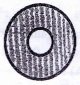
\includegraphics{du-al.png}
\end{minipage}%



\question   দুটি সমমানের ভেক্টর একটি বিন্দুতে ক্রিয়াশীল । এদের লদ্ধির মান যেকোন একটি ভেক্টরের মানের সমান । ভেক্টর দুটির মধ্যবর্তী কোণের মান কত? (Two vectors of equal magnitude are acting at a point. The value of the resultant vector is equal t the value of either of the vectors. What is the angle between the vectors?)

\begin{oneparchoices}
\choice $ 0^{\circ} $
\choice $ 90^{\circ} $
\choice $ 120^{\circ} $
\choice $ 180^{\circ} $
\end{oneparchoices}

\question একটি গাড়ি সোজা রাস্তায় স্থির অবস্থা থেকে যাত্রা শুরু করলো। কিছু সময় পরে গাড়িটি মন্দনের মাধ্যমে থেমে যায়। গড়িটি একই পথে একইভাবে যাত্রা করে পূর্ববর্তী স্থানে ফিরে আসে। নিন্মলিখিত কোন লেখচ্ত্রিটি গাড়িটির গতিকে প্রকাশ করে? (A car accelerates from rest on a straight road. A short time later the decelerates to a stop. It then returns to its original position in s similar manner. which of the following graph best describe the motion ?)

\begin{oneparchoices}
 \choice\begin{tikzpicture}
      \draw[->] (0,0) -- (2,0);
      \draw[->] (0,0) -- (0,2) ;
      \draw (0,1)node[left] {$x$};
     \draw (2,0) node[below] {$t$};
      \draw[scale=0.4,domain=0:1,smooth,variable=\x,blue] plot ({\x},{(\x)});
     \draw[scale=0.4,domain=1:3,smooth,variable=\x,blue] plot ({\x},{(2-\x)});
          \draw[scale=0.4,domain=3:4.3,smooth,variable=\x,blue] plot ({\x},{(-4+\x)});
    \end{tikzpicture}
 \choice\begin{tikzpicture}
      \draw[->] (0,0) -- (2,0);
      \draw[->] (0,0) -- (0,2) ;
      \draw (0,1)node[left] {$x$};
     \draw (2,0) node[below] {$t$};
      \draw[scale=0.5,domain=0:1.5,smooth,variable=\x,blue] plot ({\x},{(\x)});
     \draw[scale=0.5,domain=1.5:3,smooth,variable=\x,blue] plot ({\x},{(3-\x)});

    \end{tikzpicture}
\choice\begin{tikzpicture}
      \draw[->] (-1,0) -- (1,0);
      \draw[->] (-1,0) -- (-1,2) ;
      \draw (-1,1)node[left] {$x$};
     \draw (1,0) node[right] {$t$};
      \draw[scale=0.5,domain=-1.8:1.8,smooth,variable=\x,blue] plot ({\x},{3*(pow(2,-(\x*\x)))-.3});
    \end{tikzpicture}
 \choice \begin{tikzpicture}
      \draw[->] (0,0) -- (2,0);
      \draw[->] (0,0) -- (0,2) ;
      \draw (0,1)node[left] {$a$};
     \draw (2,0) node[right] {$r$};
      \draw[scale=0.5,domain=0:3.1,smooth,variable=\x,blue] plot ({\x},{sin(deg(2*\x)});
    \end{tikzpicture}
\end{oneparchoices}

\question  ইয়াং এর দ্বিচিড় পরীক্ষায় দুটি তরঙ্গের উপরিপাতনের ফলে একটি বিন্দুতে কালো ডোরা উৎপন্ন হয়। ঐ বিন্দুতে তরঙ্গদ্বয়ের দশা পার্থক্য হলো: ($ m= $ পূর্ণসংখ্যা) (Two wave superpose to give rise to dark fringe at point in Young's double slit experiment. The phase difference between the two waves at that point is :) ($ m= $ integer)

\begin{oneparchoices}
\choice শূণ্য (zero)
\choice $ 2\pi m +\dfrac{\pi}{4}$
\choice $ 2\pi m +\dfrac{\pi}{2}$
\choice $ 2\pi m +\pi $
\end{oneparchoices}

\question  যদি তড়িৎ ক্ষেত্রের প্রাবল্য $ +x $ অক্ষ বরাবর ক্রিয়া করে এবং এর মান $ E=cx^{2} $ হয়, যেখানে $ c= $ ধ্রুবক। তবে তড়িৎ বিভব $ V=? $ (If the electric field acts in the $ +x $ direction and has a magnitude given by $ E=cx^{2} $ (here $ c= $ constant), then the electric potential  $ V=? $ ) 

\begin{oneparchoices}
\choice $ -2cx $
\choice $ 2cx $
\choice $ -\dfrac{cx^{3}}{3} $
\choice $ \dfrac{cx^{3}}{3} $

\end{oneparchoices}

\question  হাইড্রোজেন পরমাণুর প্রথম বোর কক্ষে ইলেকট্রনের মোট শক্তি $ -13.6\,ev $। তৃতীয় বোর কক্ষে মোট শক্তি কত? (An electron in the first bohr orbit of the hydrogen atom has total energy of $ -13.6\,ev $. What is the total energy in the third bohr orbit? )

\begin{oneparchoices}
\choice $ -15.6\,eV $
\choice $ -3.4\,eV $
\choice $ -4.5\,eV $
\choice $ -40.8\,eV $
\end{oneparchoices}

\question শূণ্যমাধ্যমে প্রবাহমান একটি সমতল তরঙ্গমুখের বিদ্যুৎ ও চৌম্বক ক্ষেত্রের বিস্তারের অনুপাত $ \dfrac{E}{B} $ এর মান এস আই এককে হলো : (In a plane electromagnetic wave propagating in vacuum, the ratio of the amplitudes of the electromagnetic fields, $ \dfrac{E}{B} $ in SI units is: )

\begin{oneparchoices}
\choice তরঙ্গের কৌণিক কম্পাংক, $ \omega $ (Angular frequency of the wave $ \omega $)\\
\hspace*{-.3cm}\choice শূণ্যমাধ্যমে তরঙ্গদৈর্ঘ্য $ \lambda $ (the wavelength of the wave in vacuum $ \lambda $)\\
\hspace*{-.3cm}\choice  শূণ্যমাধ্যমে আলোর বেগ, $ c $ (the speed of the light in vacuum $ c $)\\
\hspace*{-.3cm}\choice  প্লাংকের ধ্রুবক, $ h $ (Planck's constant, $ h $)
\end{oneparchoices}

\question  সরণ পাওয়া যায়: (Displacement is obtained from: )

\begin{oneparchoices}
\choice বেগ-সময় লেখচিত্রের ঢাল থেকে (the slope of the velocity-time graph.)\\
\hspace*{-.3cm}\choice ত্বরণ-সময় লেখচিত্রের ঢাল থেকে (the slope of the acceleration-time graph.)\\
\hspace*{-.3cm}\choice বেগ-সময় লেখচিত্রের নিচের ক্ষেত্রফল থেকে (the area under the velocity-time graph.)\\
\hspace*{-.3cm}\choice ত্বরণ-সময় লেখচিত্রের ক্ষেত্রফল থেকে (the area under the acceleration-time graph.)

\end{oneparchoices}

\question সমদ্রুতিতে $ r $ ব্যসার্ধের বৃত্তাকার পথে ঘূর্ণায়মান একটি কণার ক্ষেত্রে নিচের চারটি লেখচিত্রের কোনটি সঠিক? (কণার ত্বরণ $ a $) (Which of the following four graph correctly represents a particle moving in a circular path of radius $ r $ at a constant speed of $ 10\,m/s $) ($ a $ is the acceleration)

\begin{oneparchoices}
 \choice\begin{tikzpicture}
      \draw[->] (0,0) -- (2,0);
      \draw[->] (0,0) -- (0,2) ;
      \draw (0,1)node[left] {$a$};
     \draw (2,0) node[right] {$r$};
      \draw[scale=0.5,domain=00:3.5,smooth,variable=\x,blue] plot ({\x},{(2.5)});
    \end{tikzpicture}
 \choice \begin{tikzpicture}
      \draw[->] (0,0) -- (2,0);
      \draw[->] (0,0) -- (0,2) ;
      \draw (0,1)node[left] {$a$};
     \draw (2,0) node[right] {$r$};
      \draw[scale=0.5,domain=00:3.5,smooth,variable=\x,blue] plot ({\x},{(\x)});
    \end{tikzpicture}
\choice\begin{tikzpicture}
      \draw[->] (0,0) -- (2,0);
      \draw[->] (0,0) -- (0,2) ;
      \draw (0,1)node[left] {$a$};
     \draw (2,0) node[right] {$r$};
      \draw[scale=0.5,domain=00:3.5,smooth,variable=\x,blue] plot ({\x},{(3.5-\x)});
    \end{tikzpicture}
 \choice \begin{tikzpicture}
      \draw[->] (0,0) -- (2,0);
      \draw[->] (0,0) -- (0,2) ;
      \draw (0,1)node[left] {$a$};
     \draw (2,0) node[right] {$r$};
      \draw[scale=0.5,domain=0.3:3.5,smooth,variable=\x,blue] plot ({\x},{(.3+(3*exp(2*(-\x+.3))))});
    \end{tikzpicture}
\end{oneparchoices}


\question   দুটি সমান্তরাল তারের মধ্যে একই মানের তড়িৎ প্রবাহিত হয় এবং তার দুটি প্রতি একক দৈর্ঘ্যে F বলদ্বারা এক অপরকে বিকর্ষণ করে । যদি প্রবাহিত তড়িৎকে দ্বিগুণ এবং তারের মধ্যেকার মধ্যবর্তী দুরত্বকে তিনগুণ করা হয় তবে প্রতি একক দৈর্ঘ্যে বলের মান হবে : (Two parallel long wires carry the same current and repel each other with force F per unit length. If both these currents are doubled and the separation between the wires are tripled, the force per unit length becomes:)

\begin{oneparchoices}
\choice $ \dfrac{2F}{3} $
\choice $ \dfrac{4F}{3} $
\choice $ \dfrac{2F}{9} $
\choice $ \dfrac{4F}{9} $

\end{oneparchoices}

\question  গ্রহের গতির ক্ষেত্রে – "একটি নক্ষত্র থেকে গ্রহকে সংযোককারী সরলরেখা সমান সময়ে সমান ক্ষেত্রফল অতিক্রম করে" - এটি কোন নীতির সরাসরি ফলাফল? (In planetary motions - \say{the line joining the star to the planet sweeps out equal areas in equal times}. This is direct principle of which principle? )

\begin{oneparchoices}
\choice শক্তির সংরক্ষণ নীতি (the conservation of energy)\\
\hspace*{-.3cm}\choice ভরবেগের সংরক্ষণ নীতি (the conservation of momentum) \\
\hspace*{-.3cm}\choice কৌণিক ভরবেগের সংরক্ষণ নীতি (the conservation of angular momentum)\\
\hspace*{-.3cm}\choice ভরের সংরক্ষণ নীতি (the conservation of mass)
\end{oneparchoices}

\end{questions}

\end{document}